
\chapter{INTRODUCTION}


Tooth decay is one of the most widespread health problems in the world. It occurs when a tooth's enamel is damaged. Cavities in the teeth caused by tooth decay can lead to tooth loss. According to a recent study, tooth decay has surpassed heart disease as the most frequent health problem worldwide, affecting almost 34.1\% of the population [2]. People in many parts of the world have limited access to dental specialists. Since caries is not life threatening, many patients with untreated caries wait until it is too late, when major complications have already occurred and treatment is too expensive. Dental cavities that go untreated can lead to pulpitis and periapical disorders [3]. However, tooth decay can be halted and the decay process reversed if diagnosed early enough. The enamel has a self-healing property. As a result, early detection of tooth decay is an important factor of treatments to prevent dental caries. It may make dental treatment more affordable for persons with lower and medium incomes.\\
Artificial Intelligence (AI) is becoming increasingly popular and widely used in medicine to diagnose and treat patients more rapidly and accurately. Deep learning (DL), an artificial intelligence (AI) method, has been used to automate decision-making processes in numerous clinical dental situations in recent years [4]. By autonomously learning from datasets containing human annotations from dental specialists, the approach, which consists of multi layer ConvNets, has already showed promising accuracy on unforeseen data.\\
The focus of this study was on identifying tooth decay in three phases. The three phases are visible change without cavitation, visible change with micro-cavitation, and visible change with cavitation. Each phase is distinct in terms of personality, patterns, and shapes. The characteristics of the stages are described as follows and illustrated in Figure 1:
\begin{enumerate}
\item Visible change without cavitation: This is the earliest stage of tooth decay, when a lesion forms on the tooth. It causes a slight darkening of the tooth's surface, which is usually white or brown [1].
\item Visible change with micro-cavitation: In this stage, demineralization continues and the tooth enamel (the uppermost layer of the tooth's structure) begins to break down.
\item Visible change with cavitation: In this stage, the dentin layer of the tooth is impacted as the tooth decay proceeds. Bacteria get inside the decaying pulp and causes infection. 
\end{enumerate}
\vspace{5pt}
\begin{figure}[H]
    \centering
    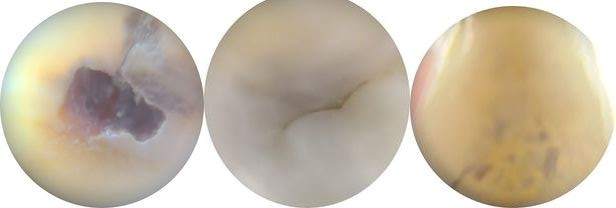
\includegraphics[scale=0.5]{10_Chapter_1/1.jpg}
    \caption{(a) Visible change without cavitation, (b) Visible change with micro-cavitation, (c) Visible change with cavitation}
    \label{Types of class}
\end{figure}
This paper offers a method for accurately predicting and classifying the three phases of tooth decay using deep learning techniques. For the automatic detection of dental decay from oral photos, we constructed a deep Convolutional Neural Network. The model classifies the presence of dental decay in a given image and uses bounding boxes to locate the findings. 
We used three different YOLO object detection models to train the dataset. In section V, the comparison study of the three has been analyzed for a better representation and understanding of the trained model's efficiency and accuracy. The rest of the paper is set out as follows: The second section covers relevant works. Section III dives into the model's training phases. Experimental setup is covered in Section IV. Section VI concludes with some ideas for the future.

